\chapter{Progettazione del sistema}

\begin{preamble}
{\em 
In questo capitolo, si esplorerà in dettaglio la progettazione dell'applicazione Android. Si esamineranno i diagrammi delle principali classi implementate nel progetto per fornire una visione completa della loro struttura. \newline \indent Successivamente, si presenterà un diagramma di sequenza che illustrerà le interazioni dinamiche tra le classi principali implementate nell'app. Questo permetterà di comprendere in dettaglio le operazioni svolte dall'applicazione durante il processo di riconoscimento degli oggetti. \newline \indent Inoltre, si descriveranno le animazioni implementate in Unity, che contribuiscono a rendere l'esperienza utente più coinvolgente e interattiva. Per completare il quadro della progettazione, si esplorerà anche la struttura del database utilizzato per memorizzare informazioni cruciali sulle bottiglie di vino. Questa parte è essenziale per garantire un recupero e una gestione efficiente dei dati all'interno dell'app Android.
}
\end{preamble}

\section{Scelte progettuali effettuate}

Nel capitolo precedente è stata fornita un'ampia panoramica degli strumenti software utilizzati, insieme alle rispettive funzionalità principali. In questa sezione, verranno descritte le versioni e le modalità di utilizzo degli strumenti. Nello specifico, questi ultimi sono:

\begin{itemize}
  \item \textit{Unity}: è stata selezionata la versione dell'editor \textit{Unity 2022.3.9f1 LTS (Long-Term-Support)} al fine di garantire maggiore stabilità, rinunciando alle ultime versioni.
  \item \textit{Vuforia Engine}: è stata impiegata la Versione \textit{10.17.4}.
  \item \textit{PolyCam}: in questo contesto, è stata scelta la \textit{Photo Mode} dell'applicazione. Sono state acquisite oltre 100 fotografie della bottiglia della Cantina Strappelli tramite uno smartphone al fine di creare un modello tridimensionale dell'oggetto, comprensivo di texture per il riconoscimento del colore e della grafica dell'etichetta della bottiglia di vino.
  \item \textit{Blender}: poiché non sono richieste funzionalità avanzate di Blender per il progetto, è stata installata l'ultima versione disponibile, ossia la Versione \textit{3.6}.
  \item \textit{Vuforia Model Target Generator}: anche in questo caso, è stata utilizzata l'ultima versione disponibile dell'applicazione, ovvero la Versione \textit{10.17.4}.
  \item \textit{OpenWeather}: nel progetto, è stata utilizzata la Versione 2.5 dell'API di OpenWeather.
\end{itemize}


\section{Diagrammi delle classi}

Un \textit{diagramma delle classi} (o \textit{Class Diagram}, in inglese) è uno dei diagrammi più comuni utilizzati nella modellazione dei sistemi orientati agli oggetti nell'ambito dell'ingegneria del software. Questo diagramma fa parte del linguaggio di modellazione \textit{Unified Modeling Language (UML)}, che è ampiamente utilizzato per rappresentare visivamente le strutture e le relazioni dei componenti di un sistema software.

Un diagramma delle classi prende, per ciascuna classe, tre sezioni principali, ovvero:

\begin{itemize}
    \item \textit{Nome della classe}: è il nome della classe, che rappresenta un concetto all'interno del sistema software.
    \item \textit{Attributi}: gli attributi sono le variabili che appartengono alla classe. Sono elencati sotto il nome della classe e possono includere tipi di dati e valori iniziali.
    \item \textit{Metodi}: i metodi sono le funzioni o i comportamenti associati alla classe. Sono elencati sotto gli attributi e mostrano i dettagli sulla firma dei metodi, inclusi i parametri e i tipi di ritorno.
\end{itemize}

\subsection{La classe IotAPICaller}

La classe \textit{IotAPICaller} è responsabile della gestione delle chiamate API per ottenere i dati provenienti dalla stazione IoT situata nel campo dell'azienda vitivinicola Strappelli. Come menzionato nel capitolo precedente, la stazione IoT carica i dati in tempo reale su una piattaforma cloud, la quale ospita un'appostia API che consente l'accesso ai dati.

L'API restituisce i dati in formato JSON, strutturati in modo simile ad una tabella di un database relazionale. Questa struttura comprende un'intestazione e un corpo di tabella, con l'aggiunta di due campi aggiuntivi, denominati \textit{status} e \textit{rows}.

La classe \textit{IotAPICaller} effettua una richiesta HTTP POST con una query SQL nel corpo della richiesta per ottenere i dati più recenti caricati dalla stazione IoT sulla piattaforma cloud.

Un esempio della struttura dei dati è riportato di seguito:

\begin{lstlisting}[caption=File JSON restituito dall'API della stazione IoT, label=lst:iotjson, captionpos=b]
 {
    "status":"succ",
    "head":
        [
            "ts",
            "coll_time",
            "temperature",
            "humidity",
            "rainfall_today",
            "rainfall_instantaneous",
            "rainfall_yesterday",
            "rainfall_total",
            "soil_temperature",
            "soil_moisture",
            "leaf_humidity",
            "leaf_temperature",
            "ext_str",
            "ext_var1",
            "ext_var2"
        ],
    "data":
        [
            [
                "2023-09-16 15:22:04.627",
                "2023-09-16 15:22:04.625",
                23.00000,
                89.90000,
                0.00000,
                0.00000,
                3.50000,
                3.50000,
                -3.50000,
                -2.50000,
                2.00000,
                25.30000,
                0.00000,
                0.00000,
                0.00000
            ]
        ],
    "rows":1
}
\end{lstlisting}

Il primo campo denominato \textit{"status"} mostra lo stato della richiesta HTTP inviata.
Il campo \textit{"head"}, come già accennato, rappresenta l'intestazione della tabella che descrive i dati; quest'ultima è composta dai seguenti campi inseriti all'interno di un array:

\begin{itemize}
    \item \textit{ts}: rappresenta un timestamp che indica quando i dati sono stati registrati.
    \item \textit{coll\_time}: rappresenta il momento in cui i dati sono stati effettivamente raccolti.
    \item \textit{temperature}: rappresenta la temperatura in gradi Celsius.
    \item \textit{humidity}: rappresenta l'umidità relativa dell'aria in percentuale. 
    \item \textit{rainfall\_today}: rappresenta la quantità di pioggia caduta durante la giornata, espressa in millimetri.
    \item \textit{rainfall\_instantaneous}: rappresenta la quantità di pioggia caduta istantaneamente al momento della raccolta dei dati espressa in millimetri.
    \item \textit{rainfall\_yesterday}: rappresenta la quantità di pioggia caduta nella giornata precedente, espressa in millimetri.
    \item \textit{rainfall\_total}: rappresenta la quantità totale di pioggia caduta fino a quel momento, espressa in millimetri.
    \item \textit{soil\_temperature}: rappresenta la temperatura del suolo in gradi Celsius.
    \item \textit{soil\_moisture}: rappresenta l'umidità del suolo, in percentuale o un'altra unità specifica.
    \item \textit{leaf\_humidity}: rappresenta l'umidità delle foglie delle piante, in percentuale o un'altra unità specifica.
    \item \textit{leaf\_temperature}: rappresenta la temperatura delle foglie delle piante in gradi Celsius.
    \item \textit{ext\_str}, \textit{ext\_var1} e \textit{ext\_var2}: questi campi contengono dati aggiuntivi in formato numerico.
\end{itemize}

Il campo \textit{data} contiene al suo interno i valori associati all'intestazione presente nel campo \textit{head}. Infine, il campo \textit{rows} contiene il numero di righe estratte dalla query SQL.

La classe IotAPICaller (Figura \ref{4fig:classDiagramIotAPICaller}) ha i seguenti attributi:

\begin{itemize}
\item \textit{txtLeafTemp}: temperatura della foglia nell'interfaccia grafica di Unity.
\item \textit{txtLeafHum}: umidità della foglia nell'interfaccia grafica di Unity.
\item \textit{txtTemp}: temperatura atmosferica nell'interfaccia grafica di Unity.
\item \textit{txtHum}: umidità atmosferica nell'interfaccia grafica di Unity.
\item \textit{txtRain}: millimetri di pioggia giornalieri nell'interfaccia grafica di Unity.
\item \textit{txtLatestUpd}: timestamp dei dati presentati nell'applicazione Unity.
\end{itemize}

\begin{figure}[h]
	\centering
	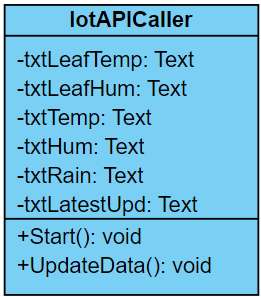
\includegraphics [width=.30\columnwidth, angle=0]
            {ClassDiagramIotAPICaller}
	\caption{Class Diagram della classe \textit{IotAPICaller}}
	\label{4fig:classDiagramIotAPICaller}
\end{figure}

Ogni variabile ha l'attributo \textit{SerializeField} per renderla privata e visibile nell'editor di Unity in modo tale da essere vista e modificata nel valore direttamente nell'interfaccia grafica, anche se il campo è dichiarato come privato.

Infine, la classe contiene i seguenti metodi:

\begin{itemize}
    \item \textit{Start}: è il primo metodo eseguito al lancio dello script nella pagina "Racconta" dell'applicazione. Inizializza correttamente una richiesta HTTP impostando l'intestazione e il corpo con la query SQL per il recupero dei dati.
    \item \textit{UpdateData}: aggiorna i dati visualizzati nell'applicazione eseguendo una chiamata API aggiuntiva.
\end{itemize}

\subsection{La classe OpenWeatherAPICaller}

La classe \textit{OpenWeatherAPICaller} (Figura \ref{4fig:classDiagramOpenWeatherAPICaller}) si occupa di gestire i dati che provengono dall'API di OpenWeather. Quest'ultima restituisce i dati in formato JSON. Un esempio è fornito di seguito:

\begin{lstlisting}[caption=File JSON restituito dall'API OpenWeather, label=lst:openweatherjson, captionpos=b]
{
    "coord":
            {
                "lon": 13.7589,
                "lat": 42.8142
            },
    "weather":
            [
                {
                    "id": 800,
                    "main": "Clear",
                    "description": "clear sky",
                    "icon": "01d"
                }
            ],
    "base": "stations",
    "main":
            {
                "temp": 299.41,
                "feels_like": 299.41,
                "temp_min": 295.96,
                "temp_max": 301.19,
                "pressure": 1016,
                "humidity": 65,
                "sea_level": 1016,
                "grnd_level": 992
            },
    "visibility": 10000,
    "wind":
            {
                "speed": 3.41,
                "deg": 62,
                "gust": 2.6
            },
    "clouds":
            {
                "all": 0
            },
    "dt": 1694272098,
    "sys":
            {
                "type": 2,
                "id": 2006527,
                "country": "IT",
                "sunrise": 1694234268,
                "sunset": 1694280450
            },
    "timezone": 7200,
    "id": 3165549,
    "name": "Torano Nuovo",
    "cod": 200
} 
\end{lstlisting}

Il file JSON presenta diversi campi tra cui:

\begin{itemize}
    \item \textit{coord}: contiene le coordinate geografiche della località; esso prende i seguenti sottocampi:
    \begin{itemize}
        \item \textit{lon}: rappresenta la longitudine del campo da monitorare.
        \item \textit{lat}: rappresenta la latitudine del campo da monitorare.
    \end{itemize}

    \item \textit{weather}: contiene informazioni sulle condizioni meteorologiche attuali; esso prende i seguenti sottocampi:
    \begin{itemize}
        \item \textit{id}: codice numerico che rappresenta il tipo di condizione meteorologica.
        \item \textit{main}: racchiude una descrizione categorica del meteo attuale.
        \item \textit{description}: descrizione più dettagliata della condizione meteo.
        \item \textit{icon}: rappresenta un'icona associata alle condizioni meteorologiche.
    \end{itemize}
    \item \textit{base}: specifica la stazione meteorologica di riferimento.
    \item \textit{main}: contiene informazioni sulle condizioni meteorologiche principali; esso prende i seguenti sottocampi:
    \begin{itemize}
        \item \textit{temp}: rappresenta la temperatura attuale in gradi Celsius.
        \item \textit{feels\_like}: è la temperatura percepita in gradi Celsius.
        \item \textit{temp\_min}: rappresenta la temperatura minima prevista in gradi Celsius.
        \item \textit{temp\_max}: indica la temperatura massima prevista in gradi Celsius.
        \item \textit{pressure}: rappresenta la pressione atmosferica in hPa.
        \item \textit{humidity}: rappresenta l'umidità relativa in percentuale.
        \item \textit{sea\_level}: rappresenta la pressione al livello del mare in hPa.
        \item \textit{grnd\_level}: rappresenta la pressione al livello del suolo in hPa.
    \end{itemize}
        
    \item \textit{visibility}: rappresenta la visibilità attuale in metri.
    \item \textit{wind}: contiene informazioni sul vento; esso prende i seguenti sottocampi:
    \begin{itemize}
        \item \textit{speed}: rappresenta la velocità del vento in metri al secondo.
        \item \textit{deg}: rappresenta la direzione del vento in gradi.
        \item \textit{gust}: rappresenta la velocità delle raffiche di vento in metri al secondo.
    \end{itemize}
    
    \item \textit{clouds}: fornisce informazioni sulle nuvole; esso prevede il seguente sottocampo:
    \begin{itemize}
        \item \textit{all}: rappresenta la copertura nuvolosa in percentuale.
    \end{itemize}
        
    \item \textit{dt}: è il timestamp Unix che rappresenta il momento in cui sono stati acquisiti questi dati meteorologici.
    \item \textit{sys}: questo campo contiene informazioni sul sistema; esso prende i seguenti sottocampi:
    \begin{itemize}
        \item \textit{type}: rappresenta il tipo di sistema.
        \item \textit{id}: rappresenta l'ID del sistema.
        \item \textit{country}: rappresenta il paese associato a questa località.
        \item \textit{sunrise}: rappresenta il timestamp Unix del sorgere del sole.
        \item \textit{sunset}: rappresenta il timestamp Unix del tramonto del sole.
    \end{itemize}
        
    \item \textit{timezone}: è il fuso orario della località in secondi rispetto all'UTC. 
    \item \textit{id}: rappresenta l'ID univoco associato alla località.
    \item \textit{name}: è il nome della località.
    \item \textit{cod}: rappresenta lo stato della richiesta HTTP.
\end{itemize}

La classe \textit{OpenWeatherAPICaller} (Figura \ref{4fig:classDiagramOpenWeatherAPICaller}) ha il compito di trasformare la stringa JSON proveniente dall'API di OpenWeather in una serie di variabili, ciascuna corrispondente a un campo del file JSON. Per svolgere questa operazione, essa fa uso di classi strutturate in modo da organizzare e incapsulare i dati relativi alle condizioni meteorologiche in una forma facilmente gestibile all'interno dell'applicazione. La classe principale, denominata \textit{WeatherData}, raccoglie tutti i dati relativi alle condizioni meteorologiche, mentre le altre classi vengono impiegate per rappresentare informazioni specifiche all'interno di questa struttura dati gerarchica.

\begin{figure}[h]
	\centering
	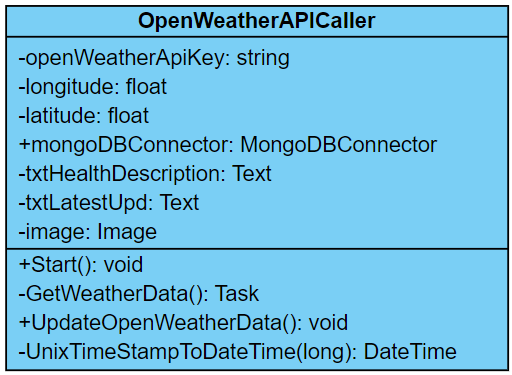
\includegraphics [width=.55\columnwidth, angle=0]
            {ClassDiagramOpenWeatherAPICaller}
	\caption{Class Diagram della classe \textit{OpenWeatherAPICaller}}
	\label{4fig:classDiagramOpenWeatherAPICaller}
\end{figure}

Le proprietà presenti nella classe \textit{OpenWeatherAPICaller} sono:

\begin{itemize}
    \item \textit{openWeatherApiKey}: contiene la chiave che consente l'utilizzo dell'API \textit{OpenWeather}.
    \item \textit{longitude}: contiene la longitudine del campo da monitorare.
    \item \textit{latitude}: contiene la latitudine del campo da monitorare.
    \item \textit{mongoDBConnector}: contiene l'istanza della classe \textit{MongoDBConnector} che si occupa di gestire la connessione con il database MongoDB (essa verrà descritta approfonditamente in seguito).
    \item \textit{txtHealthDescription}: rappresenta il testo all'interno dell'interfaccia grafica di Unity relativo alla descrizione sistetica dello stato di salute del vigneto.
    \item \textit{txtLatestUpd}: rappresenta il testo all'interno dell'interfaccia grafica di Unity relativo all'ultimo aggiornamento dei dati ottenuti dall'API \textit{OpenWeather}.
    \item \textit{image}: contiene il riferimento all'immagine presente nell'interfaccia grafica di Unity che mostra due tipologie di immagini in base allo stato del vigneto (in salute o in stato di allerta).
\end{itemize}

I metodi presenti nella classe sono riportati di seguito:

\begin{itemize}
    \item \textit{Start()}: è il metodo che viene eseguito per prima nel lancio dello script in Unity. Esso si occupa di recuperare la longitudine e latitudine dal database del campo associato alla bottiglia di vino riconosciuta.
    \item \textit{GetWeatherData()}: il metodo si occupa di effettuare la chiamata dall'API di OpenWeather per poi memorizzare i risultati nelle variabili associate a ciascun campo della stringa JSON restituita dall'API.
    \item \textit{UpdateOpenWeatherData}: aggiorna i dati provenienti dall'API di OpenWeather richiamando il metodo \textit{GetWeatherData}.
    \item \textit{UnixTimeStampToDateTime}: è un metodo che converte un timestamp Unix in una data nel formato \textit{DateTime}.
\end{itemize}

\subsection{La classe ScriptManager}

La classe \textit{ScriptManager} (Figura \ref{4fig:classDiagramScriptManager}) si occupa di gestire la sincronizzazione del testo con l'audio della recensione del sommelier.

\begin{figure}[h]
	\centering
	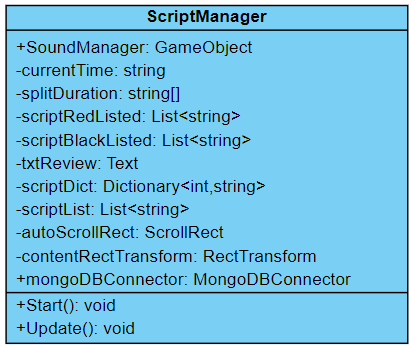
\includegraphics [width=.55\columnwidth, angle=0]
            {ClassDiagramScriptManager}
	\caption{Class Diagram della classe \textit{ScriptManager}}
	\label{4fig:classDiagramScriptManager}
\end{figure}

Gli attributi della classe sono:

\begin{itemize}
    \item \textit{SoundManager}: rappresenta l'oggetto che gestisce la riproduzione audio nella scena Unity.
    \item \textit{currentTime}: memorizza i secondi di riproduzione attuali dell'audio in riproduzione. 
    \item \textit{splitDuration}: è un array di stringhe utilizzato per suddividere la variabile \textit{currentTime} in minuti e secondi.
    \item \textit{scriptRedListed}: rappresenta una lista di stringhe per memorizzare frammenti di script che devono essere visualizzati in rosso; questi ultimi rappresentano la porzione di testo già riprodotto.
    \item \textit{scriptBlackListed}: rappresenta una lista di stringhe per memorizzare frammenti di script ancora non riprodotti.
    \item \textit{txtReview}: rappresenta un riferimento ad un componente di testo Unity utilizzato per visualizzare il testo associato allo script del sommelier.
    \item \textit{scriptDict}: rappresenta un dizionario che memorizza coppie di valori, dove la chiave è un intero (i secondi) e il valore è una stringa (il testo dello script associato a quel secondo).
    \item \textit{scriptList}: rappresenta una lista di stringhe per memorizzare l'intero script.
    \item \textit{autoScrollRect}: rappresenta un riferimento ad un componente \textit{Unity ScrollRect}. Questo attributo è serializzato in modo che possa essere assegnato nell'editor Unity. 
    \item \textit{contentRectTransform}: rappresenta un riferimento ad un componente Unity \textit{RectTransform} utilizzato per gestire il layout del contenuto all'interno del \textit{ScrollRect}.
    \item \textit{mongoDBConnector}: rappresenta un oggetto della classe \textit{MongoDBConnector} utilizzato per ottenere dati dal database MongoDB.
\end{itemize}

I metodi presenti nella classe sono i seguenti:

\begin{itemize}
    \item \textit{Start()}: questo metodo è chiamato all'avvio del \textit{GameObject}. In particolare, acquisisce il testo della recensione associata alla bottiglia riconosciuta dal database MongoDB e visualizza il testo nello script nella variabile \textit{txtRecensione}.
    \item \textit{Update()}: questo metodo è chiamato ad ogni frame dell'applicazione. Calcola il tempo corrente, identifica i frammenti di script da evidenziare in base al tempo corrente di esecuzione dell'audio della recensione, aggiorna il testo in \textit{txtRecensione}, calcola la posizione di scorrimento verticale per la visibilità del testo evidenziato e aggiorna il valore della barra di scorrimento verticale del componente \textit{autoScrollRect} in base alla posizione del testo evidenziato.
\end{itemize}

\subsection{La classe MongoDBConnector}

La classe \textit{MongoDBConnector} (Figura \ref{4fig:classDiagramMongoDBConnector}) si occupa di gestire la connessione con il database MongoDB che contiene i dati relativi al prodotto vitivinicolo identificato. La struttura del database verrà descritta in seguito.

In Figura \ref{4fig:classDiagramMongoDBConnector} è mostrato il Class Diagram della classe \textit{MongoDBConnector} di cui verranno descritti attributi e metodi presenti.

La classe presenta quattro attributi, tra cui:

\begin{itemize}
    \item \textit{apiKey}: contiene la chiave API che consente di accedere al database MongoDB.
    \item \textit{url}: l'attributo contiene l'URL dell'API di MongoDB che consente di effettuare la ricerca nel database di un particolare record con l'operazione \textit{findOne}.
    \item \textit{jsonData}: contiene un attributo che memorizza i dati JSON da inviare nel corpo della richiesta HTTP all'API di MongoDB.
    \item \textit{onDataReceived}: memorizza un attributo che contiene una funzione di callback da eseguire quando vengono ricevuti i dati dal database MongoDB.
\end{itemize}

\begin{figure}[h]
	\centering
	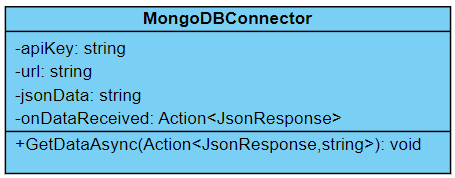
\includegraphics [width=.55\columnwidth, angle=0]
            {ClassDiagramMongoDBConnector}
	\caption{Class Diagram della classe \textit{MongoDBConnector}}
	\label{4fig:classDiagramMongoDBConnector}
\end{figure}

La classe contiene un solo metodo chiamato \textit{GetDataAsync} utilizzato per avviare un processo di recupero dei dati asincrono; tale processo accetta due parametri, ovvero:

\begin{itemize}
    \item \textit{callback}: un oggetto di tipo \textit{Action} che specifica la funzione di callback da eseguire quando vengono ricevuti dati.
    \item \textit{queryType}: una stringa che specifica il tipo di query da eseguire.
\end{itemize}

All'interno di questo metodo viene costruita una stringa di richiesta JSON in base al tipo di query richiesta; i dati pertinenti vengono ottenuti dal database MongoDB utilizzando un oggetto \textit{UnityWebRequest}. Successivamente, la risposta viene elaborata. Se la richiesta ha successo, la risposta JSON dal database viene deserializzata in un oggetto \textit{JsonResponse} e, quindi, passata alla funzione di callback specificata in \textit{onDataReceived}. Nel caso in cui la richiesta non abbia successo, viene registrato un messaggio di errore e la funzione di callback viene chiamata con un parametro nullo per indicare la presenza di un errore.

\section{Sequence Diagram}

\subsection{Introduzione}

Un \textit{diagramma di sequenza}, o \textit{Sequence Diagram}, è uno dei diagrammi \textit{UML (Unified Modeling Language)} utilizzati nella progettazione del software e nell'analisi dei sistemi. Questo tipo di diagramma viene utilizzato per visualizzare l'interazione tra oggetti o componenti all'interno di un sistema in un momento specifico nel tempo. In altre parole, esso mostra come gli oggetti comunicano tra loro e in che sequenza avvengono tali interazioni.

Di seguito, verranno illustrati alcuni elementi chiave che si possono trovare in un diagramma di sequenza:

\begin{itemize}
    \item \textit{Oggetti}: rappresentano le entità o le componenti del sistema coinvolti nell'interazione.
    \item \textit{Linee di vita}: sono linee verticali che si estendono dagli oggetti e rappresentano il periodo di tempo in cui un oggetto è attivo e coinvolto nell'interazione.
    \item \textit{Messaggi}: sono frecce orizzontali che collegano gli oggetti e rappresentano le comunicazioni o le chiamate di metodo tra gli oggetti. Possono essere annotate con informazioni aggiuntive, come i parametri dei metodi chiamati.
    \item \textit{Attivazioni}: sono rappresentate da barre verticali sopra una linea di vita e indicano il periodo in cui un oggetto sta eseguendo una determinata operazione o un metodo.
\end{itemize}

I diagrammi di sequenza sono utili per comprendere il comportamento dinamico di un sistema e per identificare potenziali problemi o inefficienze nelle interazioni tra gli oggetti. Sono ampiamente utilizzati nella fase di progettazione e analisi dei sistemi software per documentare e comunicare le interazioni tra le parti del sistema.

\subsection{Sequence Diagram del progetto}

Nel Sequence Diagram in Figura \ref{4fig:sequenceDiagram} viene mostrato il flusso di esecuzione standard che va dalla visualizzazione del menù principale fino alla pagina dedicata alla sezione desiderata dall'utente.

\begin{figure}[h]
	\centering
	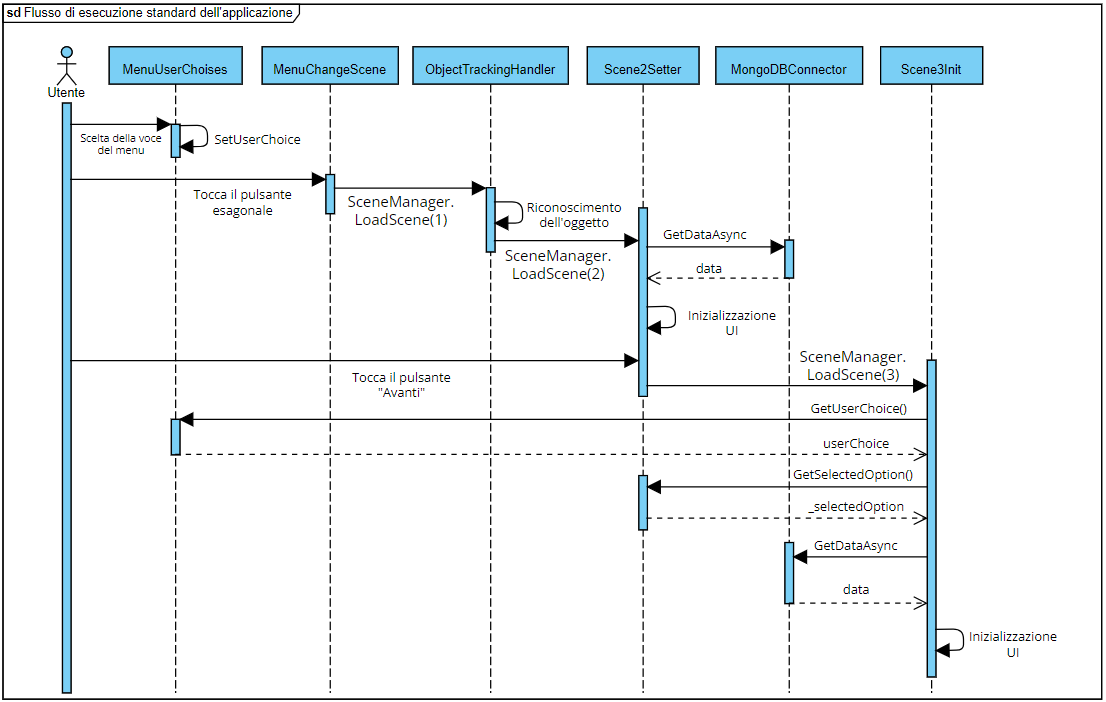
\includegraphics [width=.99\columnwidth, angle=0]
            {SequenceDiagram}
	\caption{Sequence Diagram del flusso di esecuzione principale dell'applicazione}
	\label{4fig:sequenceDiagram}
\end{figure}

Il flusso dell'applicazione procede come di seguito specificato.

Dopo che l'animazione del menù principale ha visualizzato le tre opzioni relative alle sezioni "Osserva", "Ascolta" e "Racconta", l'utente seleziona il pulsante corrispondente alla sezione di suo interesse. La classe \textit{MenuChangeChoices}, attraverso il metodo \textit{SetUserChoice}, registra il nome della sezione desiderata nella variabile \textit{userChoice}. Successivamente, l'animazione mostra il pulsante esagonale che consente di passare alla scena successiva dedicata al riconoscimento del prodotto vitivinicolo tramite il comando \textit{SceneManager.LoadScene(1)}.

L'utente accede, quindi, alla scena dedicata al riconoscimento del prodotto vitivinicolo. Una volta che l'oggetto è stato riconosciuto, la classe \textit{ObjectTrackingHandler} esegue il comando \textit{SceneManager.LoadScene(2)} per caricare la scena successiva.

Nella nuova scena, vengono richiesti i dati relativi alla bottiglia di vino riconosciuta al database MongoDB. Questi dati vengono utilizzati per popolare i campi testuali presenti nell'interfaccia grafica di Unity, come il nome della cantina e la qualità del vino.

Una volta che la scena è stata inizializzata correttamente con i dati relativi al prodotto vitivinicolo, l'utente seleziona l'annata desiderata e preme il pulsante "Avanti", il che avvia il caricamento dell'ultima scena dell'applicazione chiamata \textit{SceneManager.LoadScene(3)}.

All'avvio dell'ultima scena dell'applicazione, questa richiede alla classe \textit{MenuUserChoices} tramite il metodo pubblico \textit{GetUserChoice}, la stringa contenente la scelta effettuata dall'utente nel menu principale, precedentemente memorizzata nella variabile \textit{userChoice}. Successivamente, la classe \textit{Scene3Init} acquisisce l'annata scelta dall'utente tramite il metodo \textit{GetSelectedOption} e utilizza questi dati per popolare gli elementi dell'interfaccia grafica, richiedendo ulteriori informazioni alla classe \textit{MongoDBConnector}.


\section{Animazioni in Unity}

\subsection{Introduzione}

Le animazioni in Unity sono un elemento fondamentale per creare giochi interattivi e applicazioni. Le animazioni consentono di far muovere gli oggetti, i personaggi, le telecamere e molto altro all'interno del progetto Unity.

Di seguito, è riportata una panoramica del funzionamento delle animazioni in Unity:

\begin{itemize}
    \item \textit{Animator Controller}: è il componente principale per gestire le animazioni in Unity. Questo controller definisce gli stati, le transizioni e le regole per la riproduzione delle animazioni.
    \item Animation Clips: Un Animation Clip è un file che contiene un'animazione specifica. Puoi crearli importando file da programmi di modellazione 3D o crearli direttamente in Unity utilizzando l'Editor di animazione. Questi clip vengono poi collegati all'Animator Controller.
    \item \textit{Animator Window}: è un'interfaccia utente visuale che consente di creare e gestire le transizioni tra gli stati dell'Animator Controller. È possibile aggiungere transizioni tra diversi stati e definire le condizioni che le attivano.
    \item \textit{Layers}: gli Animator Controller possono avere più layer, che consentono di gestire animazioni sovrapposte o di priorità diverse.
    \item \textit{Blend Trees}: consentono di miscelare più animazioni in base a valori specifici, come direzione e velocità. Questi sono utili per controllare animazioni complesse.
    \item \textit{Parametri}: consentono di utilizzare parametri per controllare le transizioni tra gli stati.
    \item \textit{Scripting}: è possibile controllare l'animazione tramite script C\# in Unity.
    \item \textit{Importazione di animazioni}: è possibile importare animazioni create in programmi come Blender e collegarle all'Animator Controller.
    \item \textit{Esecuzione in tempo reale}: le animazioni in Unity possono essere eseguite in tempo reale, consentendo interazioni dinamiche con il mondo di gioco.
\end{itemize}

\subsection{Le animazioni utilizzate nel progetto}

\subsubsection{Menù principale}

In Figura \ref{4fig:menuAnimSchema}, è riportata la struttura dell'animator controller denominato \textit{Menu Controller}. Nel momento in cui l'applicazione Android viene eseguita, l'animator che si trova nello stato \textit{Entry}, attiva automaticamente l'animazione \textit{MenuFadeIn} che permette di visualizzare le tre voci del menù principale descritte nei capitoli precedenti con un effetto \textit{FadeIn} in ingresso.

Successivamente, l'applicazione rimane in attesa di un input da parte dell'utente. Quest'ultimo, nel momento in cui effettua la scelta, attiva l'animazione associata alle tre voci presenti nel menù, rispettivamente \textit{ChoiceOsserva}, \textit{ChoiceAscolta} e \textit{ChoiceRacconta}. Ciascuna di queste animazioni fa passare automaticamente allo stato \textit{Scene1\_Idle}. 

L'applicazione mostrerà un pulsante a forma di esagono che attende l'input dell'utente. Nel momento in cui il pulsante verrà premuto, si attiverà la scena dedicata al riconoscimento del prodotto vitivinicolo.

\begin{figure}[h]
	\centering
	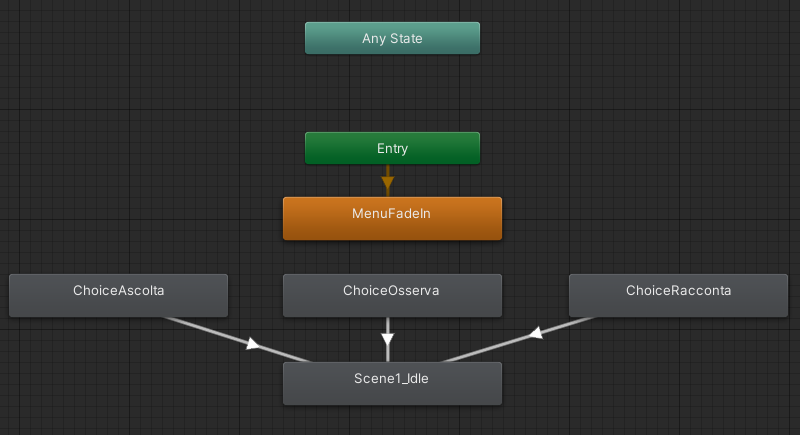
\includegraphics [width=.85\columnwidth, angle=0]
            {menuAnimSchema}
	\caption{La struttura dell'animator controller \textit{Menu Controller}} 
	\label{4fig:menuAnimSchema}
\end{figure}

\subsubsection{Scelta dell'annata}

Come già anticipato nei capitoli precedenti, una volta che il prodotto vitivinicolo è stato riconosciuto, l'applicazione carica la scena dedicata alla selezione dell'annata del vino. L'animator controller chiamato \textit{"Scene2IntroController"} (Figura \ref{4fig:scene2anim}), all'avvio della nuova scena, è nello stato \textit{Entry}, che attiva, tramite una transizione, l'animazione \textit{Scene2Intro}. Quest'ultima si occupa si effettuare lo scorrimento della finestra dal basso verso l'altro fino a metà schermo per permettere all'utente di scegliere l'annata della bottiglia di vino di suo interesse.

\begin{figure}[h]
	\centering
	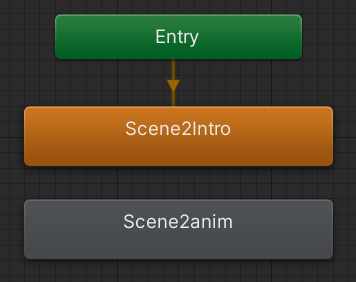
\includegraphics [width=.30\columnwidth, angle=0]
            {Scene2Anim}
	\caption{La struttura dell'animator controller "Scene2IntroController"} 
	\label{4fig:scene2anim}
\end{figure}

Dopo aver scelto l'annata, l'utente preme il pulsante "Avanti" che attiva la scena \textit{Scene2anim}; quest'ultima effettua lo scorrimento completo della finestra per creare un effetto di transizione verso l'ultima scena dell'applicazione che mostra le tre sezioni "Osserva", "Ascolta" e "Racconta".

\section{Il database MongoDB}

Il database MongoDB, come già accennato, contiene i dati relativi ai vigneti monitorati dall'azienda Trace Technologies. Ogni documento MongoDB contiene i dati di un vigneto strutturati come in Figura \ref{4fig:mongodb1}:

\begin{figure}[h]
	\centering
	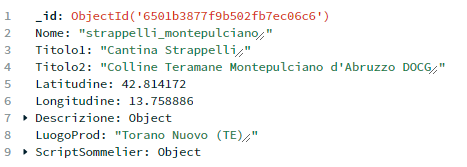
\includegraphics [width=.75\columnwidth, angle=0]
            {mongodb1}
	\caption{Documento MongoDB della cantina Strappelli}
	\label{4fig:mongodb1}
\end{figure}

Più specificatamente, i campi presenti in ogni documento MongoDB sono i seguenti:

\begin{itemize}
    \item \textit{Nome}: rappresenta il nome univoco del prodotto vitivinicolo.
    \item \textit{Titolo1}: contiene il nome che appare nelle intestazioni del prodotto vitivinicolo nelle varie sezioni dell'applicazione Android.
    \item \textit{Titolo2}: contiene le sotto-intestazioni del prodotto vitivinicolo nelle varie sezioni dell'applicazione Android.
    \item \textit{Latitudine}: memorizza la latitudine del campo associato al vigneto.
    \item \textit{Longitudine}: memorizza la longitudine del campo associato al vigneto.
    \item \textit{Descrizione}: contiene una breve descrizione delle caratteristiche del vino associato alla bottiglia riconosciuta suddivisa per annata.
    \item \textit{LuogoProd}: contiene il luogo in cui il vino viene prodotto.
    \item \textit{ScriptSommelier}: memorizza un dizionario per ogni annata, in cui ad ogni timestamp in secondi è associata una stringa di testo. Questo campo viene utilizzato nella sezione "Ascolta" descritta in precedenza per ottenere il testo sincronizzato con l'audio (Figura \ref{4fig:mongodb2}).
\end{itemize}


\begin{figure}[h]
	\centering
	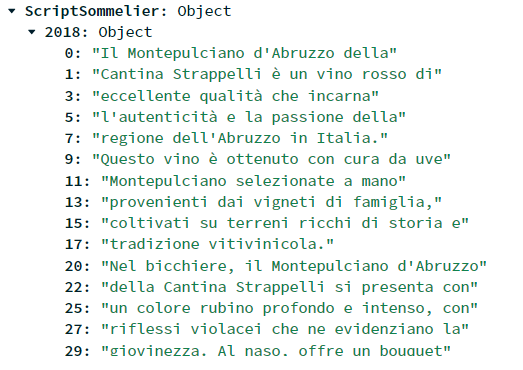
\includegraphics [width=.40\columnwidth, angle=0]
            {mongodb2}
	\caption{Struttura del campo \textit{ScriptSommelier}}
	\label{4fig:mongodb2}
\end{figure}
